\section{Proposed Approach}\label{sec:approach}

We decided to base the implementation of our concurrent priority queue on a lockfree Skiplist. A lockfree Skiplist is a good choice for a concurrent datastructure since the atomic operations are very local to 2-3 nodes and thereby the probabilty of conflicts between threads is minimized. Since our final goal was a port on to the Xeon Phi which comes with 60 cores this would be a good fit.\\
The Skiplist was implemented using C++ atomics and its {\em comapre\_and\_exchange} operation.\\
In Figure XX we have an illustration of Skiplist which essentially is a linked list with a hierarchial tree-like index structure. The index creation is probabilistic but should asymptotically lead to a structure which enables traversing to any node in $O(\log n)$.\\
MAYBE EXPLAIN some operations\\
Like most lockfree data structures we had to deal with the problem {\em predecessor-deletion} [FIND BETTER WORD, see paper]. The problem is explained in figure XX.
A common resolution is to add a delete flag to each node for lazy deletion. But this means it is necessary to do CAS operation on the {\em next} pointer and the delete flag simulatenously. Multiple options are possible: {\em Atomic Markable Reference}, Double CAS, double-width CAS, Transactional-Memory. For our implementation we used the first option and implemented a {\em Atomic Markable Reference} by using the least significant bit as a deletion flag. Thereby we are able to use the general {\em compare\_and\_exchange} operation in C++11. Since our next pointers are always alligned to 64bytes [what is the architecture doing??]. In general no issues should arise when using the least significant bit as a deletion flag.\\
Apart from the common Skiplist methods: empty(), size(), find(), remove(), insert(). We added a pop() method necessary for a priority queue and pop(k) and insert(k) for batch processing.\\


%MAYBE give complete API somewhere
\begin{lstlisting}[language=C++,basicstyle=\tt\footnotesize,captionpos=b,caption=PPQ interface,morekeywords={*, size_t}]
template <class T, class Comp> class PPQ
{
	bool empty() const;
	size_t size() const;
	bool push(const T& data);
	size_t push(T data[], int k);
	bool remove(const T& data);
	bool pop_front(T& data);
	size_t pop_front(T data[], int k);
	bool contains(T data);
	void print();
};
\end{lstlisting}

\subsection{Correcteness verification}
\label{subsec:corr_ver}
We used two different applications for verifying the correctness of our algorithm, a loseless data compression algorithm and an algorithm to find the shortest path in a graph. 
%\mypar{Huffman coding algorithm}
We implemented the Huffman coding algorithm as an initial correcteness test for our data structure implementation. This algorithm consists in two main steps. The first step is to initialize a data structure which keeps all the items sorted by their frequency. Then in a second step, it iterates until the data structure has a single element. Every iteration consists of picking the two nodes with the lowest frequency/probability, creating a parent node out of them with the sum of the children's frequencies/probabilities, inserting this new node into the data structure and assigning code zero, or one to the children, and delete them from the data structure. We compared the output of a Huffman coding algorithm using a min-heap with an implementation using our priority queue. We only compared correctness between this two implementations as this loseless compression algorithm is based on iterating linearly through the elements of the underlying data structure and no concurrent access is done.
%\mypar{Shortest path algorithm}
A shortest path algorithm performs searches over a graph to determine the a path with the least number of hops between two nodes. Thus, we tested the correctness of our application against the shortest path algorithm implementation provided by Intel TBB. This implementation uses Intel TBB concurrent priority queue by default, and we adapted to also use our priority queue. We verified the correctness of both outputs. We didn't measure any performance over these algorithms as this might have implied some specific tuning for each of them. This falls out of the scope of this project. In section~\ref{sec:exp}, we do performance evaluation against Intel TBB concurrent priority queue with specific workloads.

\subsection{Memory allocation micro-benchmark}
We performed a microbenchmark to evaluate the memory allocation process in the XeonPhi. We did three different types of mememory allocation: First, we used the primites offered by the programming language, then we used compiler hints offered by the Intel Thread Building Blocks to use its scalable allocator implementation, and finally we allocated the memory needed sequentially using compiler hints too. These options are described below.

\mypar{C++ memory allocation primitives}
These are optimized for sequential case. They were designed with two main objectives: use efficiently memory space and minimize CPU overhead. However, these objectives do not target achieving good parallel performance. Modern hardware provides larger memory sizes, but also a bigger gap between CPU and memory speed. Thus, cache locality and avoidance of false sharing play a more important role.

\mypar{Intel TBB scalable allocator}
It uses \textit{thread-private heaps} to reduce the amount of code that needs synchronization and also false sharing. Each thread allocates its own copy of heap structures and accesses it via thread-specific data (TSD) using corresponding system APIs.
The allocator gets 1MB chunks from the operating system and divides them into 16K-byte aligned blocks. Then, it places these blocks initially in a global heap of free blocks. Memory requested is not returned to the operating system (but only in large allocation cases). Thus, it can make sure that memory is reused. Additional blocks are requested if a thread does not find free objects in the blocks of its own heap and there are no available blocks in the global heap~\cite{_thefoundations,Hudson:2006:MST:1133956.1133967}.
To use the scalable allocator offered by Intel TBB we had to link two libraries:
\begin{description}
	\item[-ltbb] To use the Intel TBB library.
	\item[-ltbbmalloc] To use the scalable allocator offered by the Intel TBB library.
\end{description}
 
\mypar{Sequential allocation with compiler hints}
Every node in our skip list contains an array of pointers to the next nodes depending on the level each node belongs to. This means that parts of this array might fall into different cache lines. Thus, our data structure can suffer more from cache misses and false sharing. We designed each skip list node to contain an empty array and allocating only the pointers that it will actually need (listing~\ref{lst:freenode}). In addition to that, the usage of Intel TBB allocator helps us ensuring that these nodes will be cache-aligned (listing~\ref{lst:fn_alloc}).

\begin{lstlisting}[language=C++,basicstyle=\tt\footnotesize,captionpos=b,caption=Lock free node structure,label=lst:freenode,morekeywords={*, size_t}]
template <typename T>  struct LockFreeNode
{	
	T data;
	int	level;
	AtomicRef<LockFreeNode>	next[0];
};
\end{lstlisting}

\begin{lstlisting}[language=C++,basicstyle=\tt\footnotesize,captionpos=b,caption=Memory allocation instruction for array of atomic references,label=lst:fn_alloc, morekeywords={*, size_t}]

scalable_malloc(
sizeof(LockFreeNode) 
+ 
((arrayLength + 1) * sizeof(AtomicRef<LockFreeNode>))
)
\end{lstlisting}

\mypar{Memory allocation microbenchmnark}
We designed our microbenchmark to allocate ten million skip list nodes while using 240 threads. We measured the time it takes to complete the allocation task on the XeonPhi. When using the regular memory allocation method, we experienced really high latency but when we used Intel TBB scalable allocator we obtained a 24, and 38 times improvemente for using TBB library, and a sequential allocation with Intel TBB allocator respectively. The results are displayed on figure~\ref{fig:mem_alloc}.


% explain data + graph 
\begin{figure}
	\centering
  	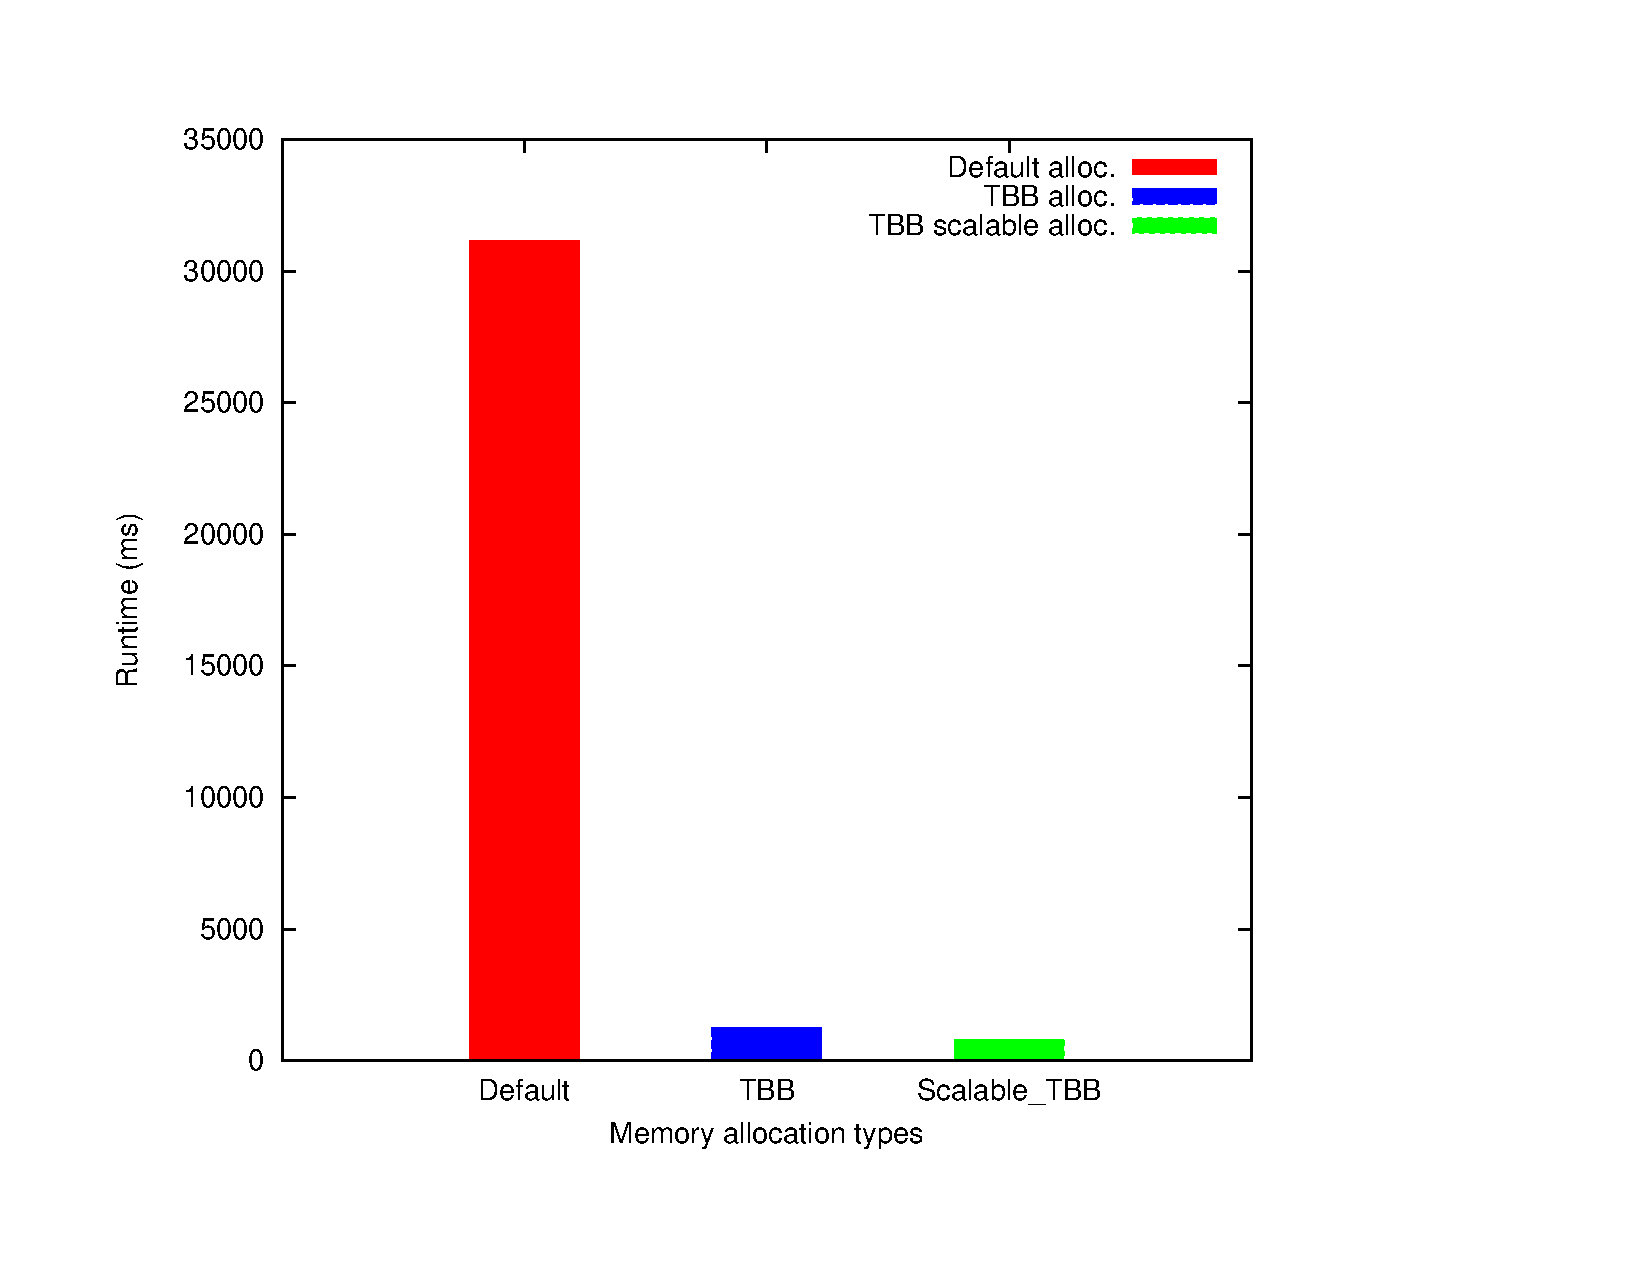
\includegraphics[scale=0.35]{../plots/mem_alloc/mem_alloc.pdf}
	\caption{Memory allocation runtime among a regular allocation, using compiler hints, and using sequential allocation with compiler hints}
	\label{fig:mem_alloc}
\end{figure}
